\chapter{ Obiektowy model dokumentu}
\label{chap:12}

  
W \hyperref[chap:11]{rozdziale 11} używaliśmy obiektów JavaScript odnoszących się do elementów \texttt{form} i \texttt{input} dokumentu HTML. Obiekty te należą do struktury o nazwie \textbf{DOM}\index{DOM} (ang. Document-Object Model — obiektowy model dokumentu)\index{obiektowy model dokumentu}. W~modelu tym reprezentację ma każdy element znajdujący się w dokumencie. Można go tam znaleźć i coś z nim zrobić.

  
Dokumenty HTML mają strukturę hierarchiczną. Każdy element (lub znacznik) z wyjątkiem głównego elementu \texttt{<html>} znajduje się w innym elemencie, który jest jego rodzicem. Element mający rodzica również może zawierać elementy potomne. Można to sobie wyobrazić, jako drzewo rodzinne.

\bigskip 
\centerline{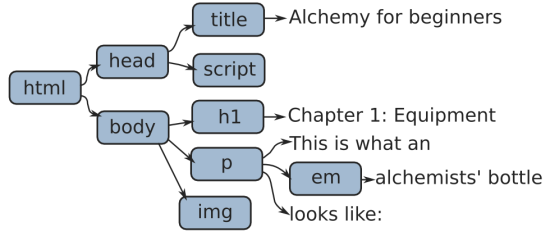
\includegraphics[width=\textwidth]{html}} 
\smallskip
  
Obiektowy model dokumentu opiera się właśnie na takiej reprezentacji dokumentu. Zwróć uwagę, że przedstawione drzewo zawiera dwa rodzaje elementów: węzły reprezentowane przez niebieskie pola i fragmenty zwykłego tekstu. Wkrótce się dowiesz, że urywki tekstu zachowują się trochę inaczej niż inne elementy. Na przykład nie mogą mieć dzieci.

  
Otwórz plik \texttt{example\_alchemy.html} zawierający dokument przedstawiony na  rysunku i powiąż go z konsolą.

  
\begin{verbatim} 
attach(window.open("/wp-content/ejs/example_alchemy.html"));
 \end{verbatim}
  
\index{document.documentElement}Dostęp do obiektu stanowiącego korzeń drzewa dokumentu, węzła \texttt{html}, można uzyskać poprzez własność \texttt{documentElement} obiektu \texttt{document}. Najczęściej jednak potrzebny jest dostęp do części \texttt{body} dokumentu dostępnej jako \texttt{document.body}\index{document.body}.



\begin{center}
• • • • •
\end{center}

  
Łącza między tymi węzłami są dostępne jako własności obiektów węzłów. Każdy obiekt DOM ma własność \texttt{parentNode}\index{parentNode}, która odnosi się do obiektu, w~którym ten obiekt się znajduje (jeżeli w ogóle ma rodzica). Ci rodzice również mają łącza wskazujące na ich dzieci, ale ponieważ dzieci może być wiele, są one przechowywane w pseudotablicy o nazwie \texttt{childNodes}\index{childNodes}.

  
\begin{verbatim} 
show(document.body);
show(document.body.parentNode);
show(document.body.childNodes.length);
 \end{verbatim}
  
Dla wygody dostępne są też łącza o nazwach \texttt{firstChild}\index{firstChild} i \texttt{lastChild}\index{lastChild} wskazujące pierwszy i ostatni element dziecko w węźle lub \texttt{null} jeśli element nie zawiera żadnego elementu.

  
\begin{verbatim} 
show(document.documentElement.firstChild);
show(document.documentElement.lastChild);
 \end{verbatim}
  
Ostatnie dwie własności to \texttt{nextSibling}\index{nextSibling} i \texttt{previousSibling}\index{previousSibling} wskazujące węzły znajdujące się „obok” określonego węzła ― są to węzły mające tego samego rodzica i znajdujące się przed lub za określonym elementem. Jeśli nie ma takiego elementu, własności zawierają wartość \texttt{null}.

  
\begin{verbatim} 
show(document.body.previousSibling);
show(document.body.nextSibling);
 \end{verbatim}


\begin{center}
• • • • •
\end{center}

  
Aby dowiedzieć się, czy wybrany węzeł reprezentuje tylko tekst czy węzeł HTML, można sprawdzić jego własność \texttt{nodeType}\index{nodeType}. Wartość \texttt{1} oznacza zwykły węzeł, a \texttt{3} węzeł tekstowy. Istnieją też inne rodzaje obiektów mające własność \texttt{nodeType}, np. obiekt \texttt{document}, którego wartość to \texttt{9}, ale najczęściej używa się jej do odróżniania węzłów tekstowych od innych.

  
\begin{verbatim} 
function isTextNode(node) {
  return node.nodeType == 3;
}

show(isTextNode(document.body));
show(isTextNode(document.body.firstChild.firstChild));
 \end{verbatim}
  
Zwykłe węzły mają własność o nazwie \texttt{nodeName}\index{nodeName} określającą typ reprezentowanego przez nie elementu HTML. Natomiast węzły tekstowe mają własność \texttt{nodeValue}\index{nodeValue} zawierającą ich treść.

  
\begin{verbatim} 
show(document.body.firstChild.nodeName);
show(document.body.firstChild.firstChild.nodeValue);
 \end{verbatim}
  
Nazwy węzłów są zawsze pisane wielkimi literami i trzeba to brać pod uwagę w wyrażeniach porównawczych.

  
\begin{verbatim} 
function isImage(node) {
  return !isTextNode(node) && node.nodeName == "IMG";
}

show(isImage(document.body.lastChild));
 \end{verbatim}


\begin{center}
• • • • •
\end{center}

  
\section*{Ćwiczenie 12.1}
\label{sec:12.1}
  
    
Napisz funkcję o nazwie \texttt{asHTML} pobierającą węzeł DOM i zwracającą łańcuch reprezentujący tekst HTML tego węzła i jego dzieci. Możesz zignorować atrybuty, tzn. wystarczy wyświetlić węzły w formie \texttt{<nazwawezla>}. Możesz używać funkcji \texttt{escapeHTML} z \hyperref[chap:10]{rozdziału 10}, aby odpowiednio dostosować treść węzłów tekstowych.

    
Podpowiedź: Rekurencja!

  
[\hyperref[sol:12.1]{pokaż rozwiązanie}]


\begin{center}
• • • • •
\end{center}

  
W istocie węzły mają coś podobnego do funkcji \texttt{asHTML}. Przy użyciu własności \texttt{innerHTML}\index{innerHTML} można pobierać tekst HTML \emph{z wnętrza} węzła, bez znaczników samego węzła. Dodatkowo niektóre przeglądarki udostępniają też własność \texttt{outerHTML}, która zawiera również sam węzeł.

  
\begin{verbatim} 
print(document.body.innerHTML);
\end{verbatim}
  
Niektóre z tych własności można też modyfikować. Zmiana własności \texttt{innerHTML} zwykłego węzła albo \texttt{nodeValue} węzła tekstowego spowoduje zmianę ich treści. Należy podkreślić, że w pierwszym przypadku podany łańcuch jest interpretowany jako HTML, podczas gdy w drugim — jako zwykły tekst.

  
\begin{verbatim} 
document.body.firstChild.firstChild.nodeValue =
  "Rozdział 1: Głęboka prawda ukryta w butelce";
\end{verbatim}
  
Albo…

  
\begin{verbatim} 
document.body.firstChild.innerHTML =
  "Znasz już element blink? <blink>Cudowny!</blink>";
\end{verbatim}


\begin{center}
• • • • •
\end{center}

  
Do tej pory dostęp do węzłów uzyskiwaliśmy przemierzając szeregi własności \texttt{firstChild} i \texttt{lastChild}. Tak też można, ale wymaga to dużo pisania i łatwo spowodować błąd. Jeśli na początku dokumentu wprowadzimy nowy węzeł, to \texttt{document.body.firstChild} nie będzie już odwoływać się do elementu \texttt{h1} i kod, w którym przyjęto takie założenie przestanie poprawnie działać. Co więcej, niektóre przeglądarki dodają węzły tekstowe dla spacji i znaków nowego wiersza znajdujących się między elementami, a inne tego nie robią. Przez to \textbf{drzewo DOM} w każdej przeglądarce może być trochę inne.

  
Alternatywnym rozwiązaniem jest przypisanie każdemu elementowi, do którego chce się uzyskać dostęp atrybutu \texttt{id}. Na przykładowej stronie obraz ma identyfikator \texttt{picture}, przy użyciu którego możemy znaleźć ten element.

  
\begin{verbatim} 
var picture = document.getElementById("picture");
show(picture.src);
picture.src = "/wp-content/uploads/ostrich.png";
\end{verbatim}
  
\index{document.getElementById}Wpisując nazwę \texttt{getElementById} nie wpisz przez pomyłkę na końcu wielkiej litery. Ponadto, jeśli musisz ją często wpisywać, grozi Ci zespół cieśni kanału nadgarstka. Ponieważ nazwa \texttt{document.getElementById} jest o wiele za długa, jak na bardzo często używaną operację, programiści JavaScript maksymalnie ją skrócili do postaci \texttt{\$}\index{\$}. Jak wiadomo znak \texttt{\$} jest w języku JavaScript literą, a więc może być używany jako nazwa zmiennej.

  
\begin{verbatim} 
function $(id) {
  return document.getElementById(id);
}
show($("picture"));
\end{verbatim}
  
Węzły DOM mają też metodę \texttt{getElementsByTagName}\index{getElementsByTagName} (kolejna fajna, krótka nazwa), która pobiera nazwę elementu i zwraca wszystkie węzły tego typu, jakie znajdują się w węźle, na rzecz którego została wywołana.

  
\begin{verbatim} 
show(document.body.getElementsByTagName("BLINK")[0]);
\end{verbatim}


\begin{center}
• • • • •
\end{center}

  
Kolejną czynnością, jaką można wykonywać na drzewie DOM jest tworzenie nowych węzłów. Dzięki temu można w dowolnym momencie dodawać elementy do dokumentu, co pozwala uzyskać różne ciekawe efekty. Niestety interfejs jest niesamowicie niezgrabny. Można go jednak trochę poprawić używając paru funkcji pomocniczych.

  
Obiekt \texttt{document} ma metody \texttt{createElement}\index{document.createElement} i \texttt{createTextNode}\index{document.createTextNode}. Pierwsza służy do tworzenia zwykłych węzłów, a druga zgodnie z nazwą do tworzenia węzłów tekstowych.

  
\begin{verbatim} 
var secondHeader = document.createElement("H1");
var secondTitle = document.createTextNode("Rozdział 2: Poważna magia");
\end{verbatim}
  
Następnie wstawimy tytuł do elementu \texttt{h1} i dodamy element do dokumentu. Najprostszym sposobem na zrobienie tego jest użycie metody \texttt{appendChild}\index{appendChild}, którą można wywołać na każdym nietekstowym węźle.

  
\begin{verbatim} 
secondHeader.appendChild(secondTitle);
document.body.appendChild(secondHeader);
\end{verbatim}
  
Nowym węzłom często przypisuje się jakieś atrybuty. Na przykład element \texttt{img} (obraz) jest bezużyteczny, jeśli nie ma atrybutu \texttt{src} wskazującego grafikę, która ma zostać wyświetlona. Większość atrybutów można traktować jako własności węzłów DOM, ale istnieją też metody \texttt{setAttribute}\index{setAttribute} i~\texttt{getAttribute}\index{getAttribute}, które umożliwiają dostęp do atrybutów w bardziej ogólny sposób:

  
\begin{verbatim} 
var newImage = document.createElement("IMG");
newImage.setAttribute("src", "/wp-content/uploads/Hiva-Oa.png");
document.body.appendChild(newImage);
show(newImage.getAttribute("src"));
\end{verbatim}


\begin{center}
• • • • •
\end{center}

  
Jednak gdy trzeba utworzyć większą liczbę węzłów, wielokrotne wywoływanie metody \texttt{document.createElement} lub \texttt{document.createTextNode}, a~następnie dodawanie atrybutów i węzłów potomnych po jednym na raz jest bardzo żmudne. Na szczęście napisanie funkcji, która wszystko za nas zrobi nie jest trudne. Zanim to zrobimy, musimy zająć się jeszcze jednym drobiazgiem ― metoda \texttt{setAttribute} poprawnie działa w większości przeglądarek internetowych, ale w Internet Explorerze może sprawiać problemy. Nazwy niektórych atrybutów HTML mają w języku JavaScript specjalne znaczenie, przez co odpowiadające im nazwy własności obiektów są nieco zmodyfikowane. Atrybut \texttt{class} ma nazwę \texttt{className}\index{className}, \texttt{for} — \texttt{htmlFor}, a~\texttt{checked} — \texttt{defaultChecked}. W Internet Explorerze metody \texttt{setAttribute} i~\texttt{getAttribute} również działają z tymi zmienionymi nazwami, zamiast używać oryginalnych nazw z HTML-a, co może być mylące. Ponadto w przeglądarce tej atrybutu \texttt{style}\index{style}, który razem z atrybutem \texttt{class} zostanie opisany w dalszej części tego rozdziału, nie można ustawiać przy użyciu metody \texttt{setAttribute}.

  
Obejście tego może wyglądać tak:

  
\begin{verbatim} 
function setNodeAttribute(node, attribute, value) {
  if (attribute == "class")
    node.className = value;
  else if (attribute == "checked")
    node.defaultChecked = value;
  else if (attribute == "for")
    node.htmlFor = value;
  else if (attribute == "style")
    node.style.cssText = value;
  else
    node.setAttribute(attribute, value);
}
\end{verbatim}
  
W każdym przypadku, w którym Internet Explorer odbiega od reszty przeglądarek robimy coś, co działa we wszystkich przypadkach. Nie przejmuj się szczegółami — jest to brzydka sztuczka, której wolelibyśmy nie stosować, ale zmuszają nas do tego niepokorne przeglądarki. Teraz możemy napisać prostą funkcję do tworzenia elementów DOM.

  
\begin{verbatim} 
function dom(name, attributes) {
  var node = document.createElement(name);
  if (attributes) {
    forEachIn(attributes, function(name, value) {

      setNodeAttribute(node, name, value);
    });
  }
  for (var i = 2; i < arguments.length; i++) {
    var child = arguments[i];
    if (typeof child == "string")
      child = document.createTextNode(child);
    node.appendChild(child);
  }
  return node;
}

var newParagraph = 
  dom("P", null, "Akapit zawierający ",
      dom("A", {href: "http://en.wikipedia.org/wiki/Alchemy"},
          "łącze"),
      " wewnątrz.");
document.body.appendChild(newParagraph);
\end{verbatim}
  
Funkcja \texttt{dom}\index{dom} tworzy węzeł DOM. Jej pierwszy argument określa nazwę elementu reprezentowanego przez tworzony węzeł, a drugi argument jest obiektem zawierającym atrybuty tego węzła lub wartość \texttt{null}, jeśli nie ma atrybutów. Dalej może znajdować się dowolna liczba argumentów, które zostaną dodane do węzła jako dzieci. Jeśli wśród nich znajdą się łańcuchy, to zostaną najpierw umieszczone w węźle tekstowym.



\begin{center}
• • • • •
\end{center}

  
Metoda \texttt{appendChild} nie jest jedynym sposobem na wstawianie węzłów do innych węzłów. Jeśli nowy węzeł nie może znajdować się na końcu swojego rodzica, można użyć metody \texttt{insertBefore}\index{insertBefore}, aby dodać węzeł przed innym węzłem dzieckiem. Nowy węzeł podaje się jako pierwszy argument, a istniejący — jako drugi.

  
\begin{verbatim} 
var link = newParagraph.childNodes[1];
newParagraph.insertBefore(dom("STRONG", null, "great "), link);
 \end{verbatim}
  
Jeśli wstawi się gdzieś węzeł mający już rodzica (\texttt{parentNode}), węzeł ten automatycznie zostanie usunięty z dotychczasowego miejsca ― żaden węzeł nie może występować w drzewie dokumentu więcej niż raz.

  
Gdy trzeba zastąpić węzeł innym, należy użyć metody \texttt{replaceChild}\index{replaceChild}, która jako pierwszy argument przyjmuje nowy węzeł, a jako drugi — stary.

  
\begin{verbatim} 
newParagraph.replaceChild(document.createTextNode("luźne "),
                          newParagraph.childNodes[1]);
\end{verbatim}
  
W końcu za pomocą metody \texttt{removeChild}\index{removeChild} usuwa się węzły potomne. Zwróć uwagę, że wywołuje się ją na \emph{rodzicu} węzła, który ma zostać usunięty i przekazuje się jej element potomny jako argument.

  
\begin{verbatim} 
newParagraph.removeChild(newParagraph.childNodes[1]);
\end{verbatim}


\begin{center}
• • • • •
\end{center}

  
\section*{Ćwiczenie 12.2}
\label{sec:12.2}
  
    
Napisz wygodną funkcję \texttt{removeElement}\index{removeElement} usuwającą przekazany jej w argumencie węzeł DOM z węzła nadrzędnego.

  
[\hyperref[sol:12.2]{pokaż rozwiązanie}]


\begin{center}
• • • • •
\end{center}

  
Podczas tworzenia nowych węzłów i przenoszenia istniejących należy pamiętać o następującej zasadzie: węzłów nie można wstawiać do dokumentu innego niż ten, w którym zostały utworzone. Oznacza to, że jeśli są dodatkowe ramki lub otwarte okna, nie można pobrać części dokumentu z jednego z tych obiektów i przenieść go do innego oraz węzły utworzone przy użyciu metod jednego obiektu \texttt{document} muszą pozostać w tym dokumencie. Niektóre przeglądarki, a konkretnie Firefox, nie przestrzegają tej zasady, przez co kod ją łamiący w Firefoksie zadziała.


\begin{center}
• • • • •
\end{center}

  
Przykładem użycia funkcji \texttt{dom} w jakimś pożytecznym celu jest program pobierający obiekty JavaScript i tworzący z nich tabelę\index{tabela}. W języku HTML tabele tworzy się przy użyciu elementów, których nazwy zaczynają się od litery „t”, np.:

  
\begin{verbatim} 
<table>
  <tbody>
    <tr> <th>Drzewo</th> <th>Kwiaty  </th> </tr>
    <tr> <td>Jabłoń</td> <td>Białe   </td> </tr>
    <tr> <td>Koral </td> <td>Czerwone</td> </tr>
    <tr> <td>Sosna </td> <td>Brak    </td> </tr>
  </tbody>
</table>
\end{verbatim}
  
Elementy \texttt{tr} reprezentują wiersze tabeli. Elementy \texttt{th} i \texttt{td} to komórki, przy czym \texttt{td} to zwykłe komórki, a \texttt{th} to komórki nagłówka, których zawartość lekko się wyróżnia. Element \texttt{tbody} (ang. table body — treść tabeli) nie jest wymagany w samym języku HTML, ale musi być użyty, gdy tabelę tworzy się z węzłów DOM, ponieważ Internet Explorer nie wyświetla tabel utworzonych bez tego elementu.


\begin{center}
• • • • •
\end{center}

  
\section*{Ćwiczenie 12.3}
\label{sec:12.3}
  
    
Funkcja \texttt{makeTable} przyjmuje jako argumenty dwie tablice. Pierwsza zawiera obiekty JavaScript, które mają być wstawione do tabeli, a druga — łańcuchy określające nazwy kolumn tej tabeli i własności obiektów, które mają zostać pokazane w tych kolumnach. Na przykład poniższe wywołanie tworzy wcześniej pokazaną tabelę:

    
\begin{verbatim} 
makeTable([{Drzewo: "Jabłoń", Kwiaty: "Białe"},
           {Drzewo: "Koral",  Kwiaty: "Czerwone"},
           {Drzewo: "Sosna",  Kwiaty: "Brak"}],
          ["Drzewo", "Kwiaty"]);
 \end{verbatim}
    
Napisz tę funkcję.

  
[\hyperref[sol:12.3]{pokaż rozwiązanie}]


\begin{center}
• • • • •
\end{center}

  
Z tematem języka HTML i obiektowego modelu dokumentu ściśle powiązane są kaskadowe arkusze stylów\index{arkusz stylów}. Jest to obszerna dziedzina, której nie sposób wyczerpująco opisać w tej publikacji, ale dzięki znajomości arkuszy stylów w języku JavaScript można robić wiele ciekawych rzeczy. Dlatego poniżej znajduje się opis podstawowych zagadnień.

  
Kiedyś jedynym sposobem na zmienianie wyglądu elementów HTML było przypisywanie im dodatkowych atrybutów albo umieszczanie ich w innych elementach, np. \texttt{center} aby wyśrodkować treść albo \texttt{font} aby zmienić właściwości czcionki. Gdy chciały się, aby wszystkie akapity albo tabele w dokumencie wyglądały w określony sposób, \emph{każdemu elementowi tego typu} trzeba było dodać kilka atrybutów. To powodowało, że dokumenty były pełne niepotrzebnych znaczników oraz strasznie trudno się je pisało i modyfikowało.

  
Oczywiście ludzie to pomysłowe stworzenia i szybko wymyślili rozwiązanie tego problemu. Arkusze stylów to narzędzie do pisania instrukcji w rodzaju „w tym dokumencie wszystkie akapity mają być drukowane czcionką Comic Sans i mieć różowy kolor, a wszystkie tabele mają mieć grube zielone obramowanie”. Instrukcje te wpisuje się w jednym miejscu na początku dokumentu lub w osobnym pliku i mają one zastosowanie do całego dokumentu. Poniżej znajduje się przykładowy arkusz stylów, który wypośrodkowuje treść nagłówków i nadaje im rozmiar 22 punktów oraz definiuje opisane wcześniej ustawienia czcionki i koloru pisma dla wszystkich akapitów należących do klasy brzydal.

  
\begin{verbatim} 
<style type="text/css">
  h1 {
    font-size: 22pt;
    text-align: center;
  }

  p.ugly {
    font-family: Comic Sans MS;
    color: purple;
  }
</style>
\end{verbatim}
  
Z arkuszami stylów związane jest pojęcie klas\index{klasa}. Jeśli na stronie znajdują się różne rodzaje akapitów, np. brzydkie i ładne, to nie należy definiować jednego stylu dla wszystkich elementów \texttt{p}, tylko użyć klas, aby je rozróżnić. Powyższy arkusz stylów zostanie zastosowany tylko do takich akapitów:

  
\begin{verbatim} 
<p class="brzydal">Lustereczko, lustereczko...</p>
\end{verbatim}
  
To właśnie tych klas dotyczy własność \texttt{className}\index{className}, o której krótko nadmieniłem przy opisie funkcji \texttt{setNodeAttribute}. Za pomocą atrybutu \texttt{style}\index{style} można dodać arkusz stylów bezpośrednio do elementu. Na przykład poniższa instrukcja definiuje czteropikselowe jednolite obramowanie dla elementu obrazu.

  
\begin{verbatim} 
setNodeAttribute($("picture"), "style",
                 "border-width: 4px; border-style: solid;");
\end{verbatim}


\begin{center}
• • • • •
\end{center}

  
Technologia kaskadowych arkuszy stylów jest o wiele bardziej skomplikowana. Niektóre style są dziedziczone przez węzły potomne po rodzicach i~reagują ze sobą nawzajem na wiele różnych sposobów, ale z punktu widzenia programisty posługującego się drzewem DOM, najważniejsze jest, aby wiedzieć, że każdy węzeł DOM ma własność \texttt{style}, za pomocą której można manipulować jego stylem oraz że jest kilka rodzajów stylów, przy użyciu których można zmusić węzły do robienia niezwykłych rzeczy.

  
Własność \texttt{style} odnosi się do obiektu zawierającego własności dla wszystkich elementów tego stylu. Możemy np. ustawić zielony kolor obramowania obrazu.

  
\begin{verbatim} 
$("picture").style.borderColor = "green";
show($("picture").style.borderColor);
\end{verbatim}
  
Zwróć uwagę, że w arkuszach stylów słowa są oddzielane łącznikiem, np. \texttt{border-color}, natomiast w JavaScripcie każde nowe słowo od drugiego rozpoczyna się wielką literą, np. \texttt{borderColor}.

  
Bardzo praktycznym stylem jest \texttt{display: none}. Za jego pomocą można czasowo ukryć wybrany węzeł: gdy własność \texttt{style.display}\index{style.display} jest ustawiona na \texttt{none}, element nie jest wyświetlany w przeglądarce, mimo że istnieje. Później \texttt{display} można ustawić na pusty łańcuch, aby spowodować pojawienie się elementu.

  
\begin{verbatim} 
$("picture").style.display = "none";
 \end{verbatim}
  
A teraz odzyskujemy nasz obrazek:

  
\begin{verbatim} 
$("picture").style.display = "";
 \end{verbatim}


\begin{center}
• • • • •
\end{center}

  
Kolejnym rodzajem stylów, które można wykorzystać na wiele ciekawych sposobów są style pozycjonujące. W prostym dokumencie HTML wszystkie elementy są rozmieszczane na ekranie przez przeglądarkę internetową ― każdy element jest ustawiany obok lub pod elementem znajdującym się przed nim w kodzie źródłowym i węzły z zasady nie nakładają się nawzajem.

  
\index{style.position}Jeśli jednak węzłowi ustawi się styl \texttt{position} na \texttt{absolute}, to zostaje on wyjęty z tzw. układu normalnego (ang. normal flow). Nie zajmuje więcej miejsca w dokumencie, tylko jakby pływa nad nim. Jego położenie można ustawiać za pomocą własności \texttt{left} i \texttt{top}. Można to wykorzystać na wiele sposobów, od zmuszenia węzła do podążania za kursorem po tworzenie okien zasłaniających resztę strony.

  
\begin{verbatim} 
$("picture").style.position = "absolute";
var angle = 0;
var spin = setInterval(function() {
  angle += 0.1;
  $("picture").style.left = (100 + 100 * Math.cos(angle)) + "px";
  $("picture").style.top = (100 + 100 * Math.sin(angle)) + "px";
}, 100);
 \end{verbatim}
  
Jeśli nie znasz się na trygonometrii, to musisz mi uwierzyć na słowo że kosinusa i sinusa używa się do obliczania współrzędnych punktów na obwodzie okręgu. Dziesięć razy na sekundę zmienia się kąt położenia obrazu i obliczane są nowe współrzędne. Częstym błędem popełnianym przy takiej pracy jest zapominanie o dodaniu jednostki \texttt{px} do wartości. W większości przypadków brak jednostki oznacza, że styl nie zadziała, a więc trzeba dodać \texttt{px} (piksele), \texttt{\%} (procenty), \texttt{em} (1em oznacza szerokość litery \texttt{M}) lub \texttt{pt} (punkty).

  
(pozwólmy obrazkowi spocząć…)

  
\begin{verbatim} 
clearInterval(spin);
\end{verbatim}
  
Miejsce uważane ze punkt 0,0 do określania pozycji zależy od tego, gdzie w dokumencie znajduje się węzeł. Jeśli węzeł znajduje się w innym węźle mającym własność \texttt{position: absolute} lub \texttt{position: relative}, to punktem zerowym jest lewy górny róg tego węzła. W pozostałych przypadkach jest nim lewy górny róg dokumentu.



\begin{center}
• • • • •
\end{center}

  
Jeśli przestudiowałeś wszystkie przykłady przedstawione w tym rozdziale i może sam też coś zrobiłeś, to dokument, w którym pracujesz został mocno sponiewierany. Może prawię morały, ale muszę Ci powiedzieć, że nie powinieneś tego robić z prawdziwymi stronami. Czasami może Cię kusić, żeby zastosować jakieś ruchome błyskotki. Ale oprzyj się tej pokusie albo Twoje strony staną się nieczytelne albo nawet będą powodować zawieszanie się przeglądarek.